``Joining points'' is a single-player game. To play it, choose two integers greater than two and call them $g$ and $r$. Then draw four points at the vertices of a square making the top two points green and the bottom two points red. Draw green points and red points inside the square taking care that no three points, including the four initial ones, are in the same line. Continue until the total number of
green points equals $g$ and the total number of red points equals $r$.

After the board is drawn, start joining points. Any two points can be joined by a line segment as long
as:
\begin{itemize}
\item The two points to be joined are of the same color, and 
\item The line segment joining the points does not intersect any other previously drawn line segment (other than at the endpoints).
\end{itemize}

Two points $u$ and $v$ are said to be in the same component if it is possible to traverse from point $u$ to point $v$ using the line segments already drawn.

You win the game if you get all the green points in one component using exactly $g - 1$ line segments, and all the red points in another component using exactly $r - 1$ line segments. It can be proven that if the points are drawn as described above, then there is always a way to win the game.

You will be given a square board of size $s$ with $g$ green and $r$ red points whose coordinates are represented by integer pairs $(x_i, y_i)$. Green points are numbered from $1$ to $g$ with the top-left point at $(0, s)$ being 1, the top-right at $(s, s)$ being 2, and interior points ranging from $3$ to $g$ in arbitrary order.
Red points are numbered from $1$ to $r$ with the bottom-left point at $(0, 0)$ being 1, the bottom-right at $(s, 0)$ being 2, and interior points ranging from $3$ to $r$ in arbitrary order.

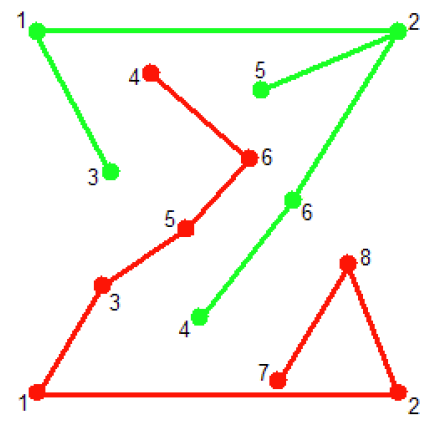
\includegraphics{points.png}

The figure shows a sample game all the green points are joined into one component and all the red points are joined into another component.

You can see that no three points are in the same line, and that no two line segments intersect each other except at their endpoints.

Write a program that, given the coordinates of the $g$ green points and the coordinates of the $r$ red points, decides how to draw $g - 1$ green line segments and $r - 1$ red line segments so that all of the green points are in the same component, all of the red points are in another component, and no two line segments intersect each other.

